\chapter{Pruebas}
\label{cap:pruebas}

\section{Módulo primero de encadenamiento entre preguntas y respuestas}
Veamos algunos ejemplos de cómo funciona el primer acercamiento a un chatbot inteligente que pregunta con algo de sentido. A continuación se muestra la primera pregunta y la respuesta del interrogado:
\begin{itemize}
	\item[] IA: ¿Quiénes son las personas más importantes de tu vida?
	\item[] Tú: Mi familia y concretamente mis padres y mi hermano
\end{itemize}

En la siguiente código se muestra el análisis que hace el módulo de cálculo de la mejor siguiente pregunta:

\begin{verbatim}
¿Hay algún momento que te gustaría volver a vivir?
0
¿Cuál es tu sexo?
[[momento, gustaría, volver, vivir]]
{'familia', 'padre', 'hermano'}
{'volver', 'vivir', 'momento', 'gustar'}
-----------------------------------------------
¿Dónde viviste cuando eras pequeño?
0
¿Cuál es tu sexo?
[[viviste, pequeño]]
{'familia', 'padre', 'hermano'}
{'pequeño', 'vivistar'}
-----------------------------------------------
¿Has vivido en algún lugar diferente cuando eras pequeño?
0
¿Cuál es tu sexo?
[[has, vivido, lugar, pequeño]]
{'familia', 'padre', 'hermano'}
{'lugar', 'pequeño', 'vivir'}
-----------------------------------------------
¿Cómo se llaman tus padres?
0
¿Cuál es tu sexo?
[[llaman, padres]]
{'familia', 'padre', 'hermano'}
{'padre', 'llamar'}
-----------------------------------------------
¿Si tienes hermanos, Cómo se llaman?
1
¿Cómo se llaman tus padres?
[[tienes, hermanos, llaman]]
{'familia', 'padre', 'hermano'}
{'llamar', 'tener', 'hermano'}
-----------------------------------------------
¿Cómo era la casa dónde viviste de pequeño?
1
¿Cómo se llaman tus padres?
[[casa, viviste, pequeño]]
{'familia', 'padre', 'hermano'}
{'pequeño', 'casa', 'vivistar'}
\end{verbatim}

%\begin{figure}[h]
	%\centering
	%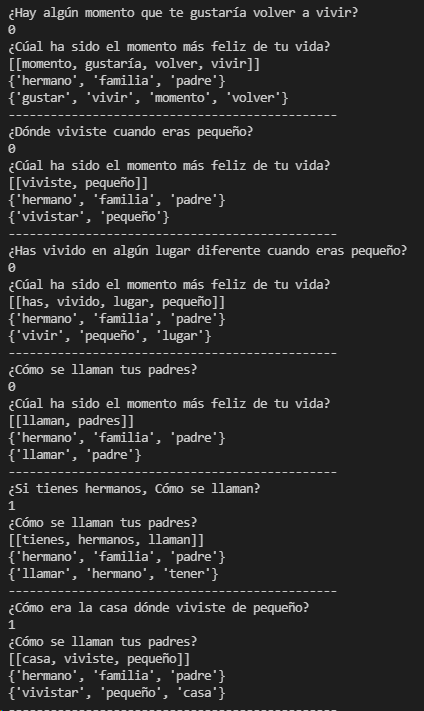
\includegraphics[scale=0.35]{Imagenes/Vectorial/modulo_encadenamiento_preguntas_respuestas_analisis}
	%\caption{}
	%\label{fig:moduloencadenamientopreguntasrespuestasanalisis}
%\end{figure}

En el código podemos observar el análisis de varias posibles preguntas. La separación entre preguntas se marca con una fila de guiones. En cada apartado nos encontramos con la posible pregunta, después el número de lemas que han coincidido en preguntas anteriores, la pregunta que hasta el momento va ganando como candidata a ser preguntada, las palabras más relevantes de la posible pregunta entre corchetes, los lemas de la respuesta entre llaves y los lemas de la posible pregunta entre llaves. Las tres primeras preguntas no serán elegidas como candidatas a ser preguntadas porque no coincide ningún lema de la respuesta con los lemas de la posible pregunta, es decir, no mejora el número de coincidencias. Cuando llega a la cuarta pregunta, ``¿Cómo se llaman tus padres?'' va a encontrar una coincidencia de tal forma:

\begin{itemize}
	\item[] Lemas de la respuesta: \hspace{2cm} \{hermano, familia, padre\} 
	\item[] Lemas de la posible pregunta: \hspace{0.8cm} \{llamar, padre\}
\end{itemize}

Como podemos observar el lema ``padre'' coincide en ambas, es decir, en esta posible pregunta encontramos una coincidencia. Como el número de coincidencias es mejor que 0, la pregunta candidata ``¿Cuál ha sido el momento más feliz de tu vida?'' se sustituye por la pregunta ``¿Cómo se llaman tus padres?''. Es por esto que cuando analizamos el resto de posibles preguntas, no encontramos ninguna que sea mejor porque no superan el número de coincidencias en lemas. En conclusión, esta será la siguiente pregunta que se le plantee al usuario, la cual tiene relación con la que se había hecho anteriormente. 

\section{Módulo primero de clasificación de respuestas en etapas de vida y en sentimientos}



